\chapter{Oxygen Reduction in \Nm{}}
\label{chap:oxygenreduction}
\section{Aerobic Reduction of Oxygen}
\subsection{Introduction}
The first dataset I used in my iterative approach to parameter estimation was of a simple oxygen reduction experiment carried out in aerobic conditions. This dataset is the simplest biologically as under aerobic conditions and without the presence of any microaerobic substrates (nitrite or nitric oxide) the only respiratory pathway that is active is the oxygen reducing one. Additionally, the other parts of a respiratory chain influence the oxygen reducing pathway either by competing for electrons, or chemically inhibiting it. The relevant portions of the ETC are shown graphically in Figure \ref{fig:o2_resp_chain}.

\begin{figure}[tbp]
	\centering
	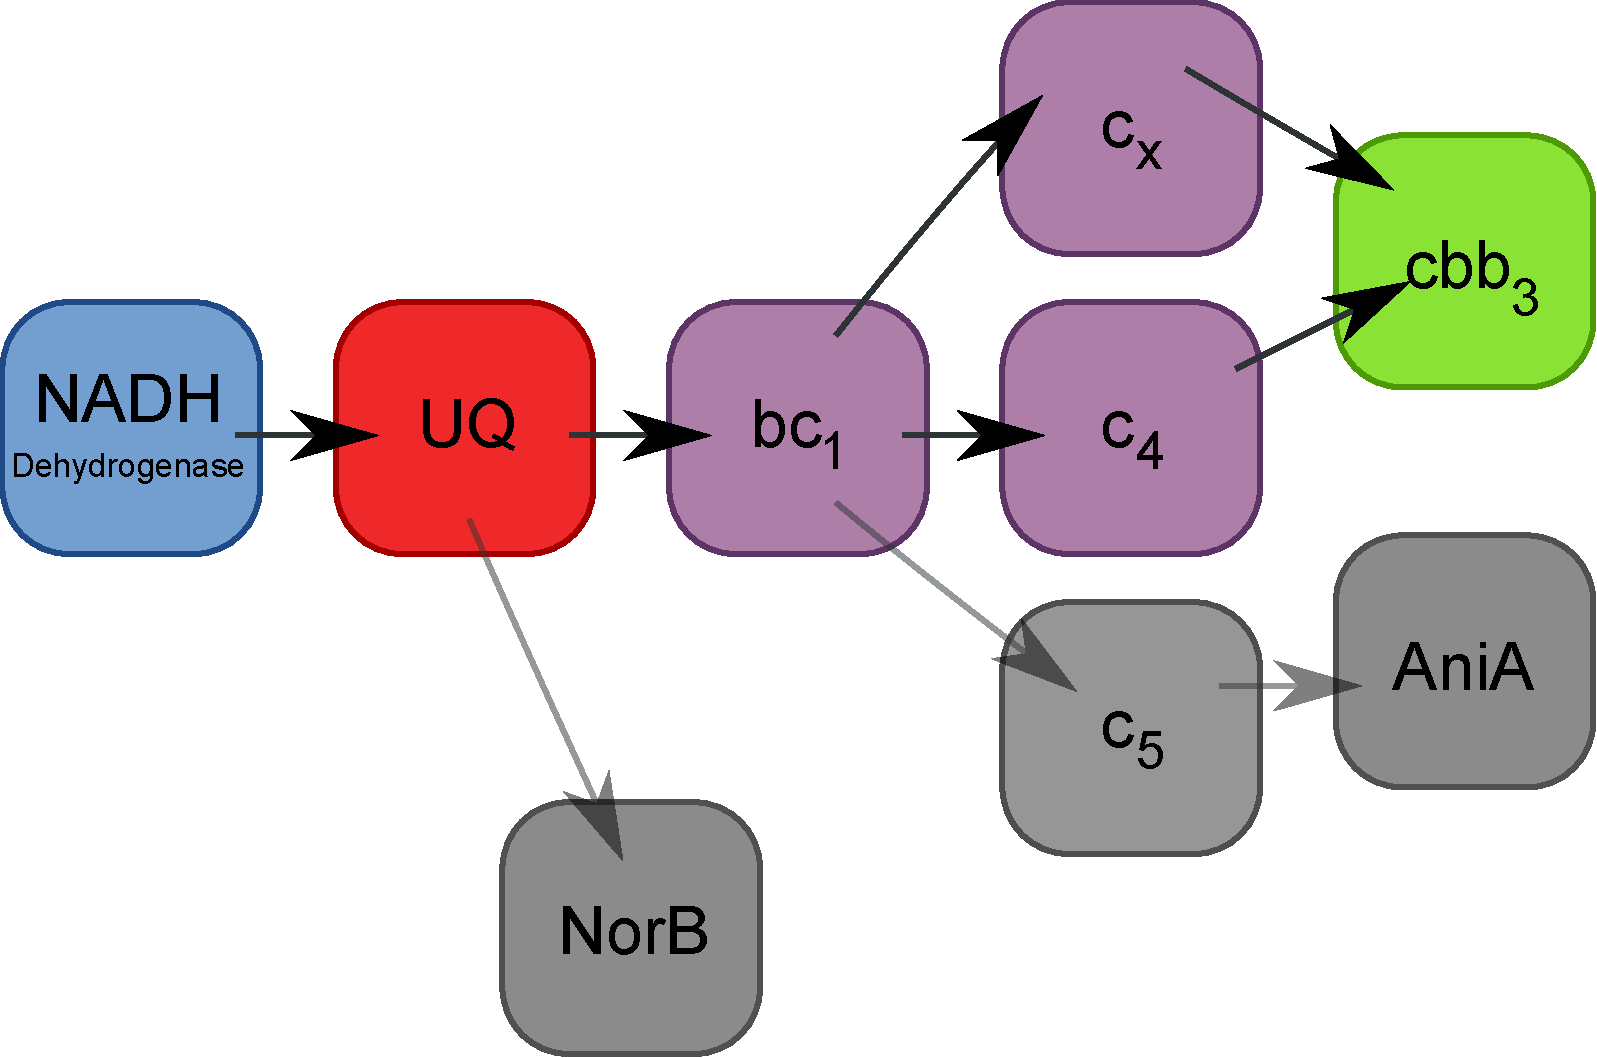
\includegraphics[width=14cm]{05-oxygenreduction/data/o2_resp_chain.pdf}
	\caption[Oxygen reducing electron transport chain of \Nm{}]{{\bf Oxygen reducing electron transport chain of \Nm{}.} This shows the complete electron transport chain of \Nsm{} with the components irrelevant to oxygen reduction greyed out. In the mathematical model all of the purple elements (cytochromes) are amalgamated into one entity.
	\label{fig:o2_resp_chain}}
\end{figure}

The equations that describe this portion of the ETC are:
\begin{eqnarray*}
\frac{d[O_2]}{dt} & = & \beta(1-[O_2]/K_O) - k_{1}[C_a][O_2]\\
\frac{d[Q_a]}{dt} & = & g([Q] - [Q_a]) - l_3[Q_a]([B] - [B_a]) - f[Q_a]([X]-[E])\\
\frac{d[E]}{dt} & = & -k_3([C] - [C_a] - [C_X])[E]  - m_3([A] - [A_a])[E] + f[Q_a]([X]-[E])\\
\frac{d[C_a]}{dt} & = & k_3([C] - [C_a] - [C_X])[E] - k_{1}[C_a][O_2] - k_5[C_a][NO]
\end{eqnarray*}
These equations describe the change in concentration of oxygen over time, which is the experimentally observable value, the reduction state of the quinone pool and the reduction state of the cytochrome ``pool''. This portion of the model involved 13 parameters and variables which I tried to estimate (the model actually contains 17 such parameters and variables, but under these conditions the remaining 4 are set to 0 as they are related to nitrite reduction effects).

\subsection{Experimental Results}
Generation of oxygen reduction datasets required the growth of MC58 (wild-type \Nsm{}) in aerobic conditions until mid log-phase growth had been achieved. This corresponds to an $\mathrm{OD}_{600}$ of 0.3-0.9 and usually required an incubation period of roughly 3 hours. Once the required cell density had been obtained, I transferred the culture to the oxygen electrode chamber and recorded the oxygen concentration as the culture respired. At this point the cells are only using whatever amount of oxygen is presently dissolved in the culture medium in addition to that diffusing in through the cap (negligible). Once the culture had used up all its dissolved oxygen, I removed the electrode chamber cap and aerated the culture media using a Pastuer pipette. This restores oxygen levels throughout the culture and allows the bacteria to continue respiring in aerobic conditions. In many cases if the culture is allowed to become completely anaerobic for a prolonged period of time, the bacteria will die, evidenced by a subsequent lack of oxygen reduction, however this is not always the case as shown in Figure \ref{fig:repeat_oxy_with_delay}. It is therefore advisable to aerate the culture before the oxygen level reaches zero. A typical oxygen reduction plot is shown in Figure \ref{fig:oxy_repeatable_chl}. This is split into individual reduction sections, which can then be used as input data for parameter estimation.

The experiments used to generate data for oxygen reduction are highly repeatable and consistently generate the same basic result of a linear reduction of oxygen with time.
\begin{figure}[tbp]
 \centering
 %trim = l b r t
 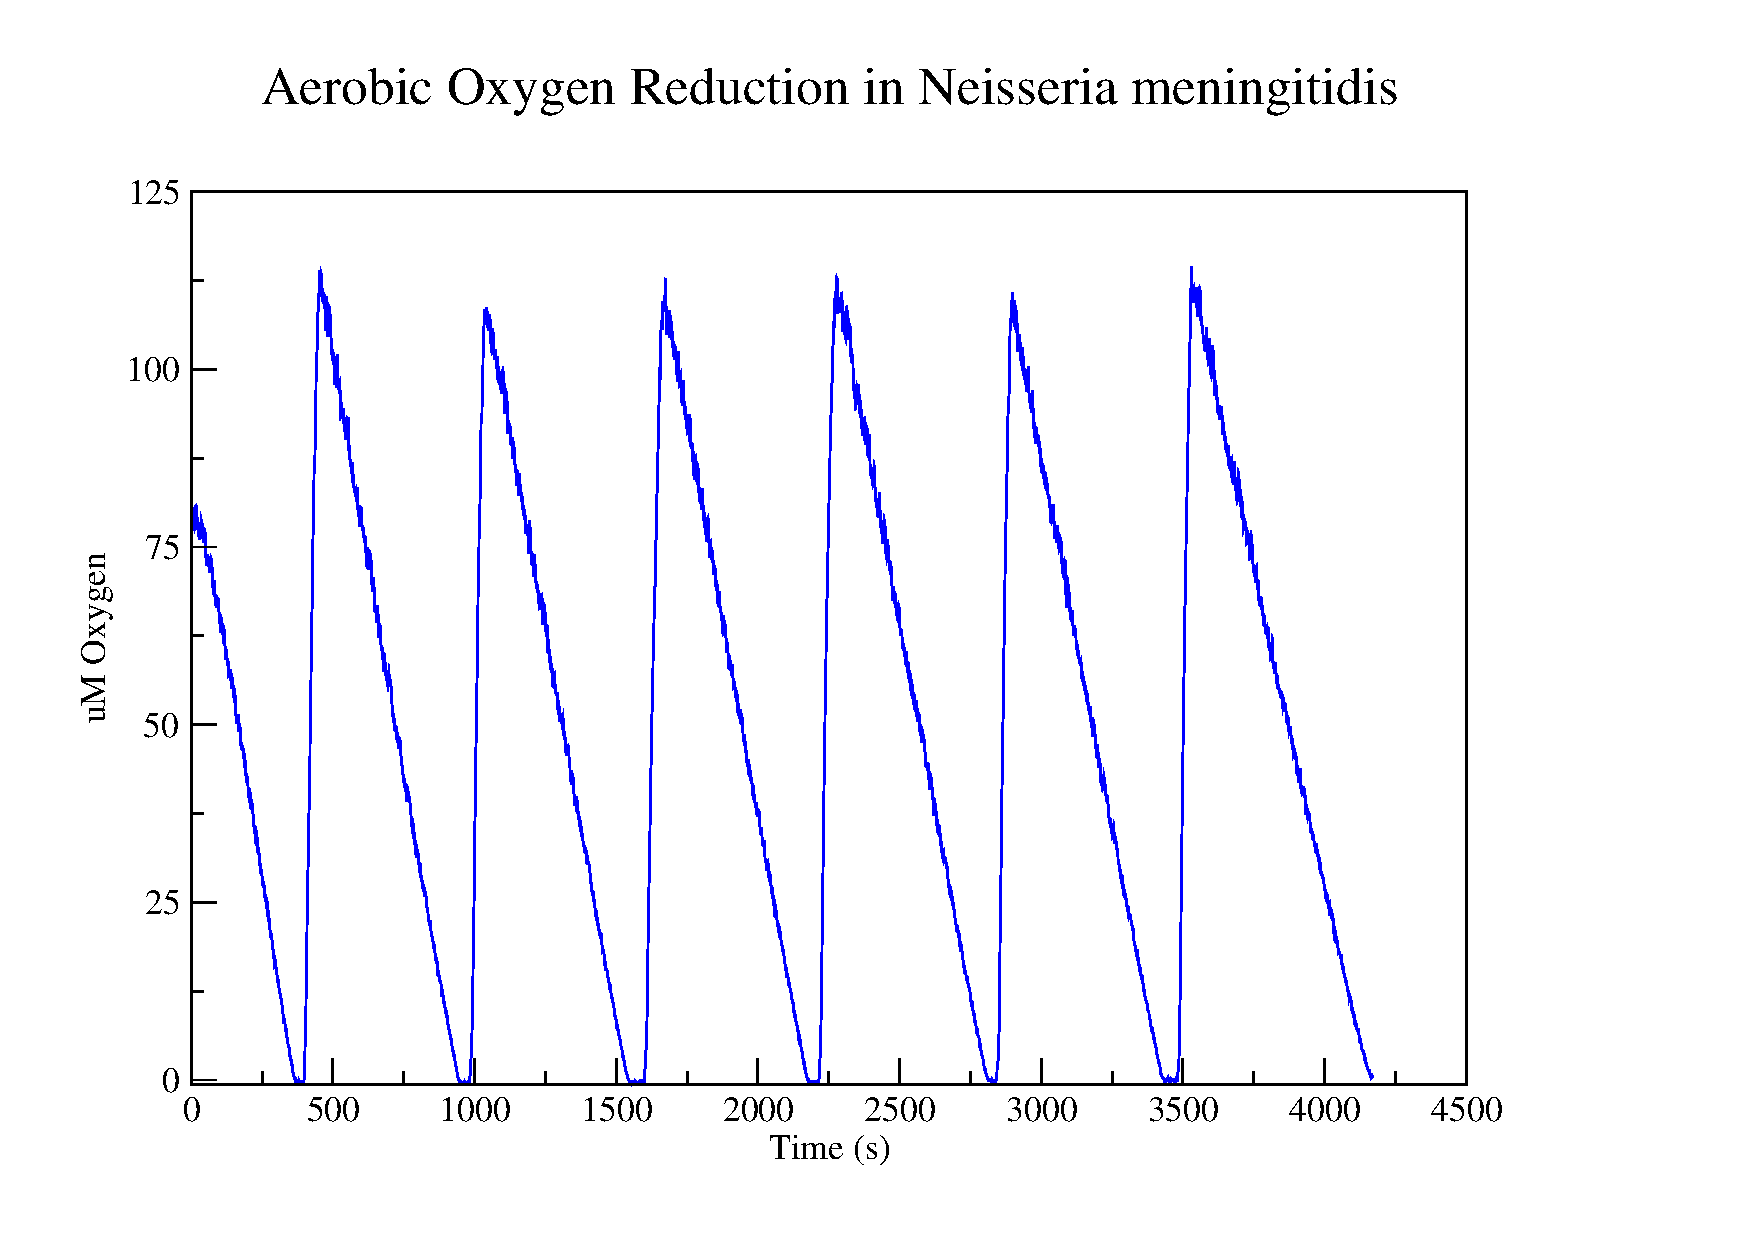
\includegraphics[width=14cm, trim=75px 50px 125px 25px]{./05-oxygenreduction/data/repeatable_o2.pdf}
 % mc58-chl-o2-util.pdf: 842x595 pixel, 72dpi, 29.70x20.99 cm, bb=0 0 842 595
 \caption[Highly repeatable oxygen reduction]{{\bf Highly repeatable oxygen reduction.} This shows an oxygen reducing culture being repeatedly aerated after oxygen depletion with very similar rates of subsequent oxygen reduction
 \label{fig:oxy_repeatable_chl}}
\end{figure}


\begin{figure}[tbp]
 \centering
 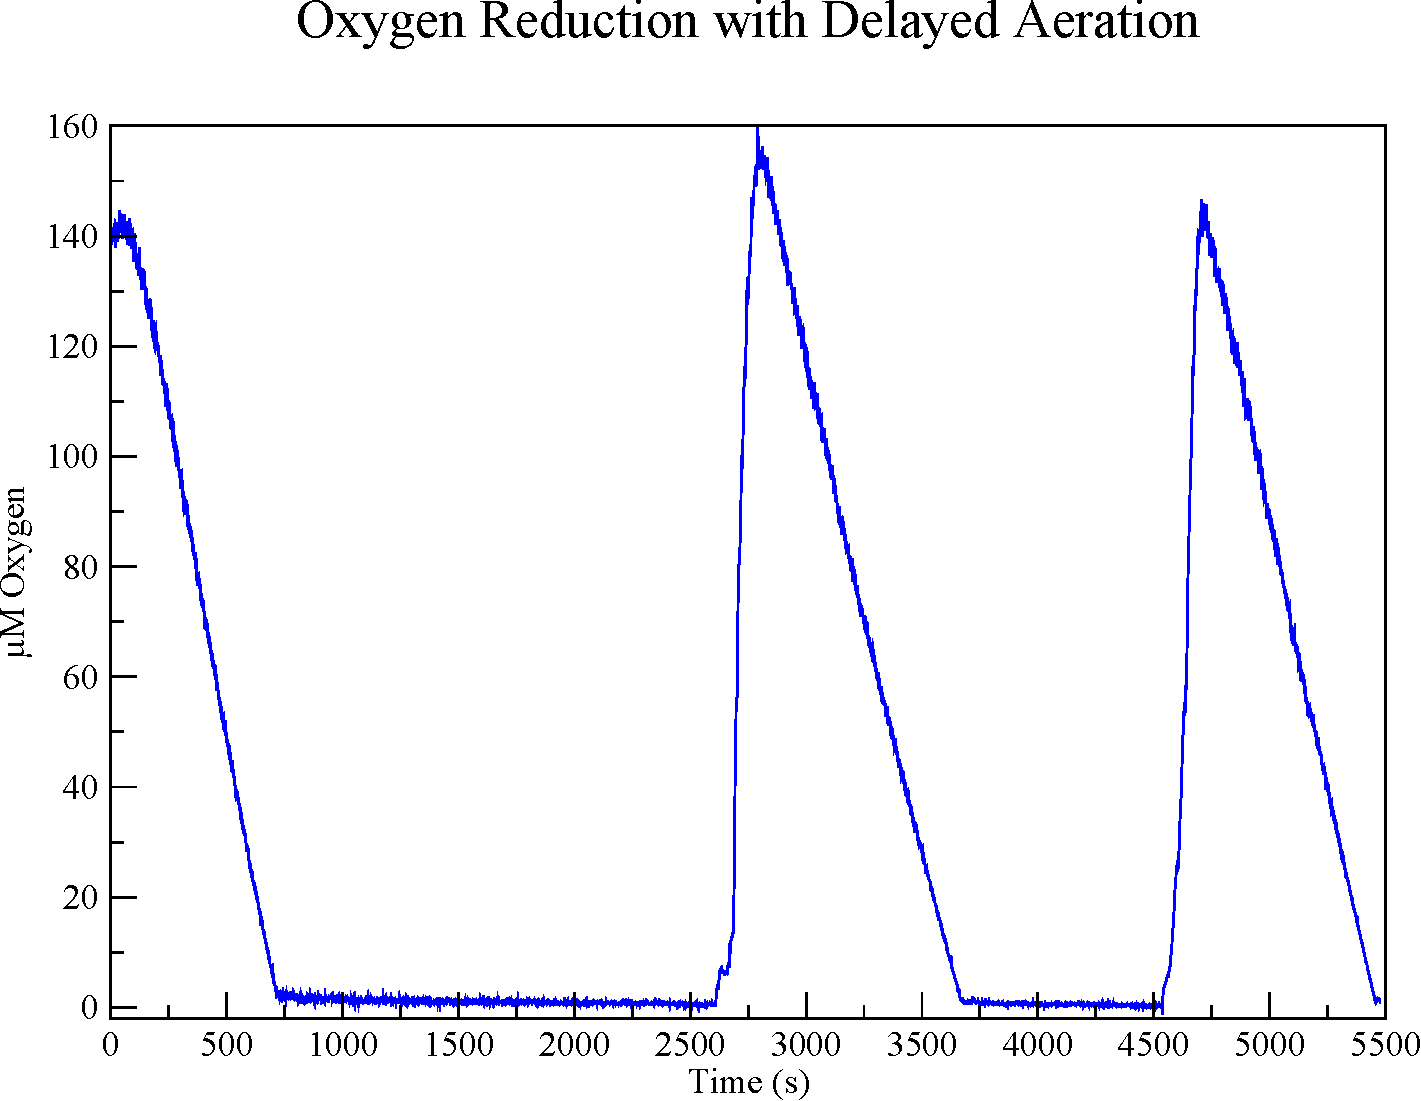
\includegraphics[width=14cm, trim=75px 50px 125px 25px]{./05-oxygenreduction/data/o2_delay.pdf}
 % repeatable-oxygen-utilisation-in-mc58.png: 640x480 pixel, 72dpi, 22.58x16.93 cm, bb=0 0 640 480
 \caption[Aerating oxygen reducing cultures with significant delay]{{\bf Aerating oxygen reducing cultures with significant delay.} The oxygen reducing ability of \Nm{} can be robust as evidenced by the 1000s delays between aeration with no change in subsequent respiration rate. Also of note is that nitric oxide concentration is not changing, suggesting that reduction of nitrite is not occurring either.
 \label{fig:repeat_oxy_with_delay}}
\end{figure}

\subsubsection{Generation of Prior Probability Distributions}
In accordance with the integrative scheme I introduced in Chapter \ref{chap:paramest}, I attempted to estimate the distributions of the parameters involved in modelling these data. In order to do this I needed to create probability distributions to act as priors to feed into the estimation system as this is required for a Bayesian approach. These probability distributions were generated from data obtained in the published literature, which is described in Chapter \ref{chap:model}, and preliminary experimental data. I assumed that all the prior probabilities would be normally distributed, therefore the distributions I used were created under the following scheme:
\begin{itemize}
	\item Where the literature value had bounds associated with it (i.e. published with $\pm{}$ values), I assumed that the bounds covered $3 \sigma$ of the normal distribution. This essentially assumes that 99.7\% of the distribution falls within the given bounds.
	\item Where the literature value has no bounds associated with it (i.e. published as a single figure), I assumed that a range of $\pm 10\%$ was covered by $3 \sigma$ of the normal distribution. This means that 99.7\% of the distribution falls within $\pm 10\%$ of the given value.
	\item Where there are no literature values available, the value was estimated based on preliminary experimental data and no bounds were associated. In this case the prior was free to be perturbed giving it an effective range of $0 < x < \infty$.
\end{itemize}
With reference to the above, the initial probability distributions used to start the Monte-Carlo run are shown in Figure \ref{fig:oxypriors}. As can be seen, very little information is readily available in the literature to populate the model.

%lbrt
\begin{figure}[tbp]
 \centering
 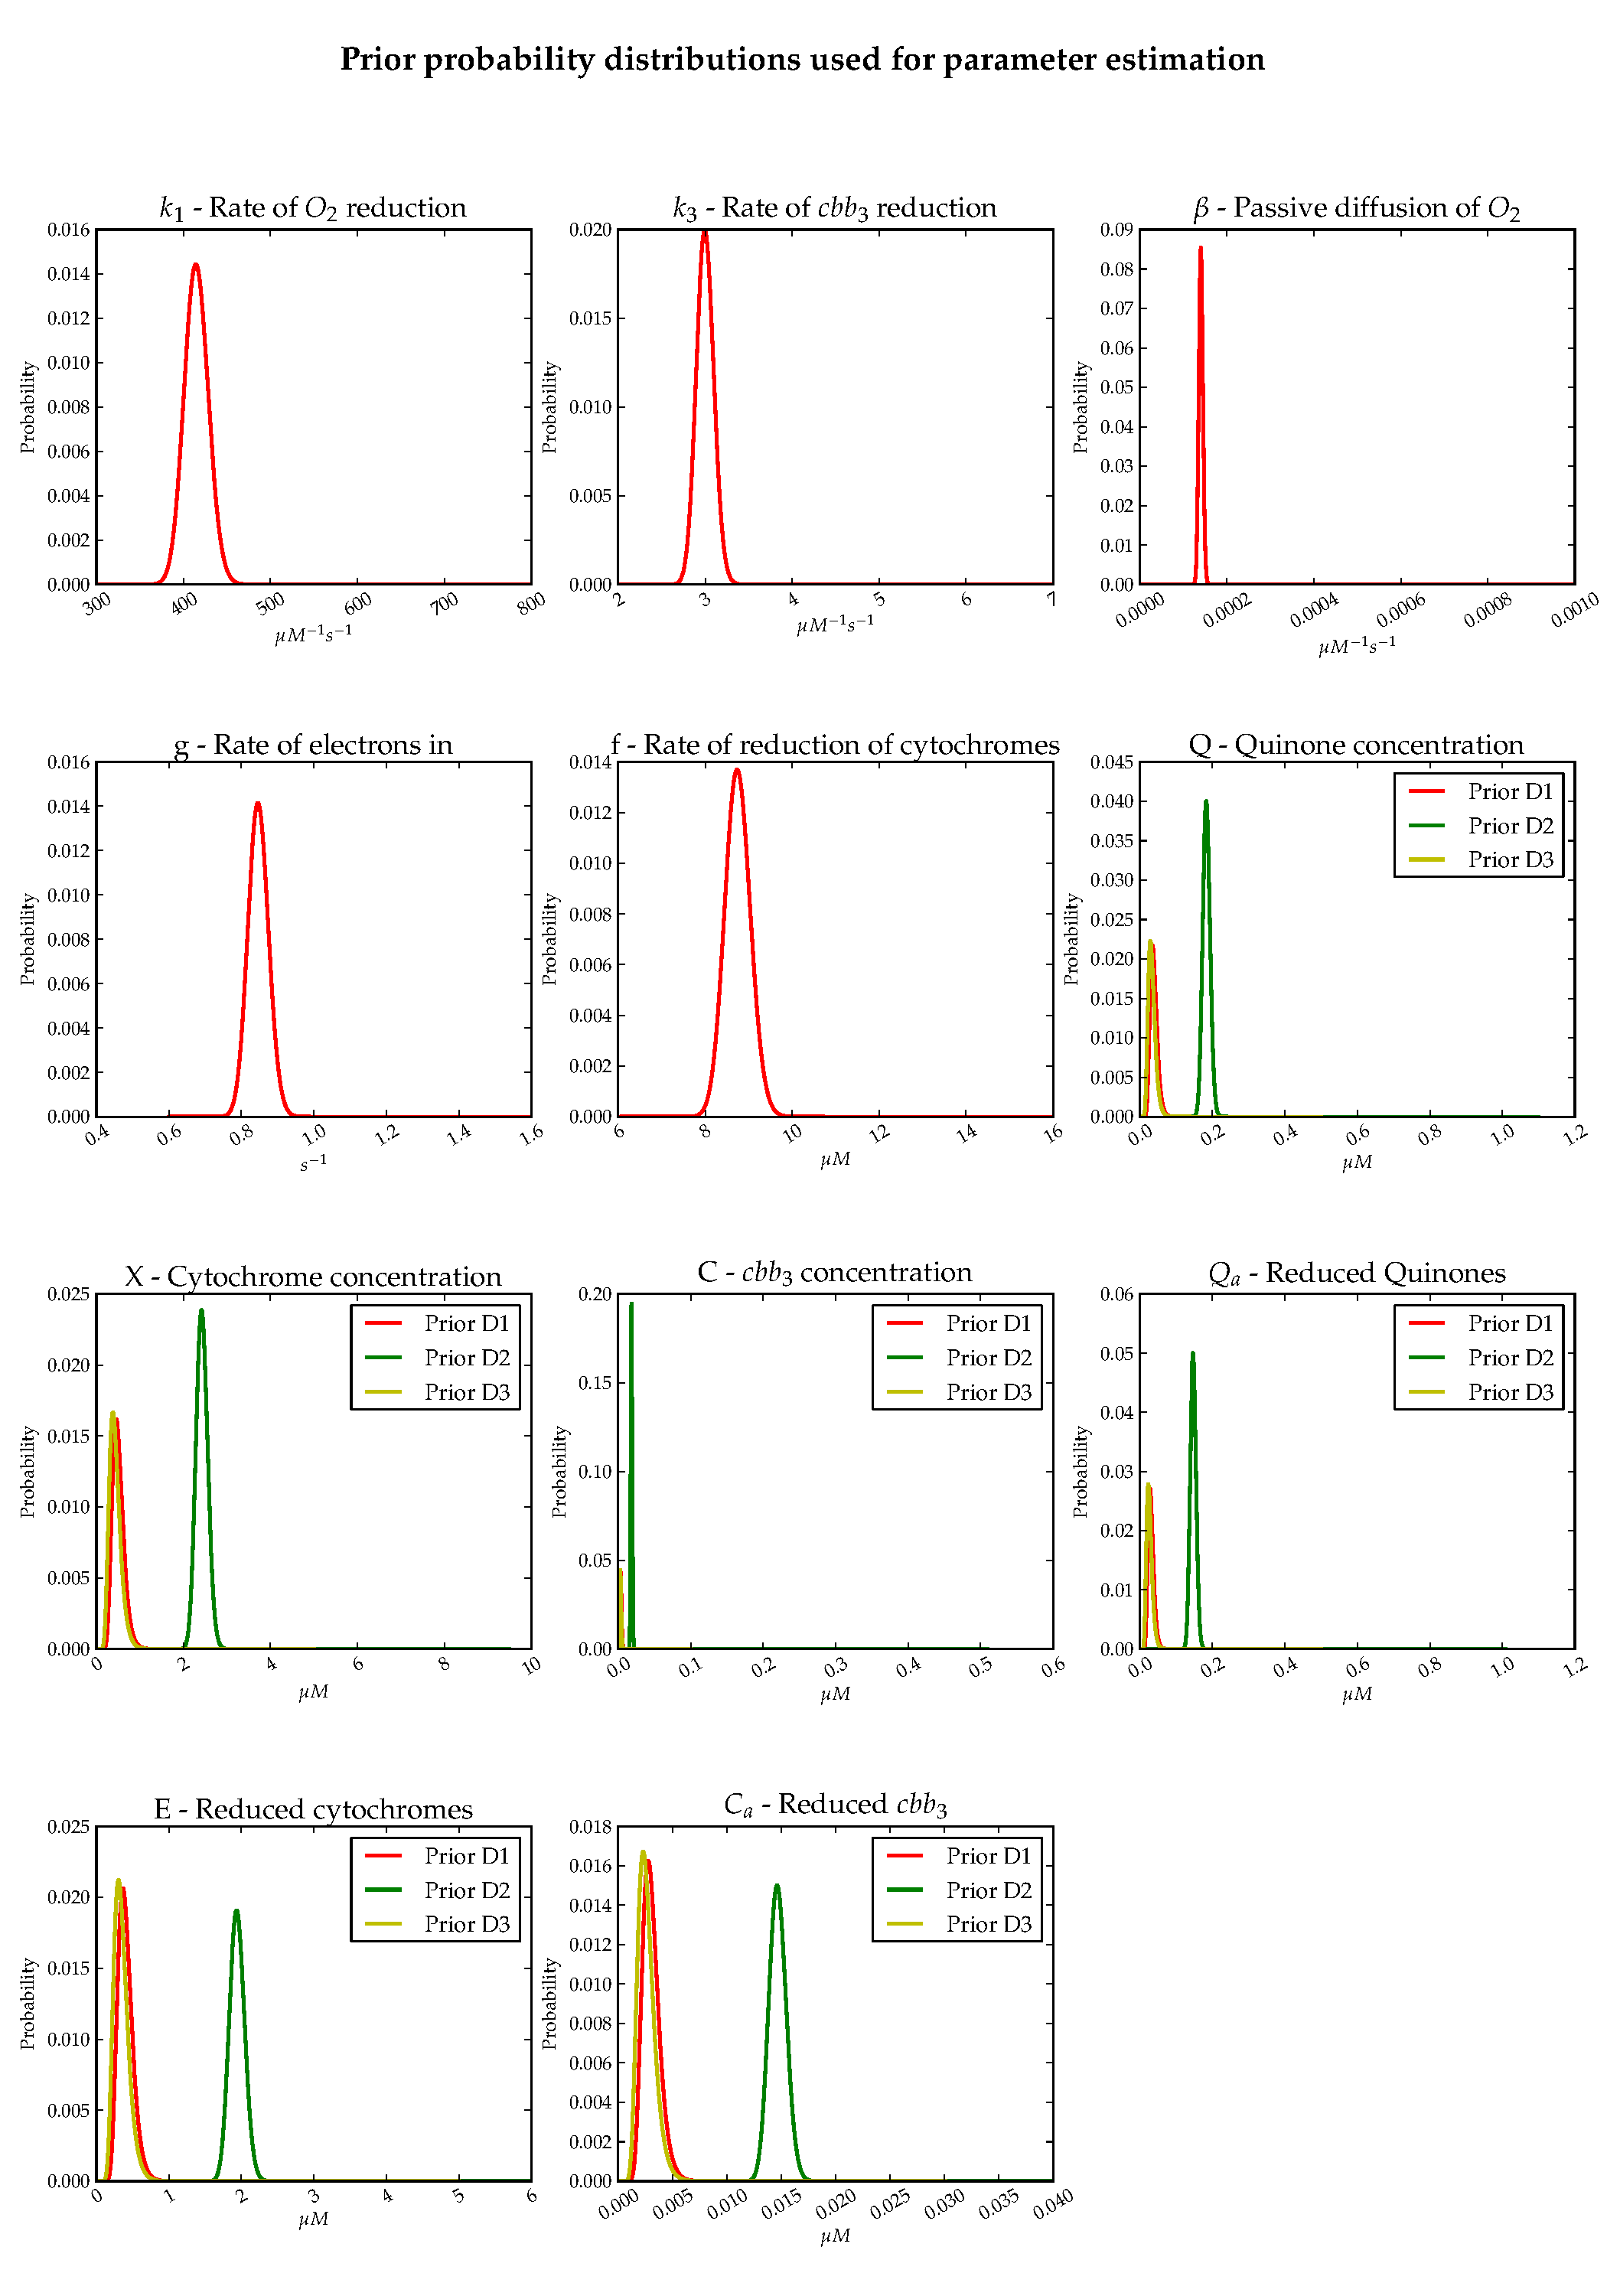
\includegraphics[width=15cm, trim=0cm 0cm 0cm 0cm]{./05-oxygenreduction/data/priors.pdf}
 % priors.pdf: 1008x1008 pixel, 72dpi, 35.56x35.56 cm, bb=0 0 1008 1008
 \caption[Prior probability distributions for oxygen reduction]{{\bf Prior probability distributions for oxygen reduction}. These are the probability distributions used as priors by the parameter estimation algorithm. Where no values were available in the literature, the probability distribution represents a flat prior from 0 to $\infty$ with the initial value being determined by preliminary experiment.
 \label{fig:oxypriors}}
\end{figure}

\subsubsection{Parameter Estimation Results}
The parameter estimation process produces a large amount of output data which can be processed. Included in these data are the best simulation results from each run. Best is defined here as the simulation with the lowest fitness value, i.e. the one with the closest match to the experimental data. For the oxygen reduction training datasets, of which there are 3, each was run 20 times for 20,000 iterations. This lower iteration count was chosen as a compromise between execution time and statistical accuracy. In fact given that the burn-in time for these runs was relatively short, 20,000 iterations still provides plenty of data. A representative example of the simulated data is shown in Figure \ref{fig:o2sim}. This figure was generated from the set of parameters that produced the most fit output compared to the input dataset.

%lbrt
\begin{figure}[tbp]
 \centering
 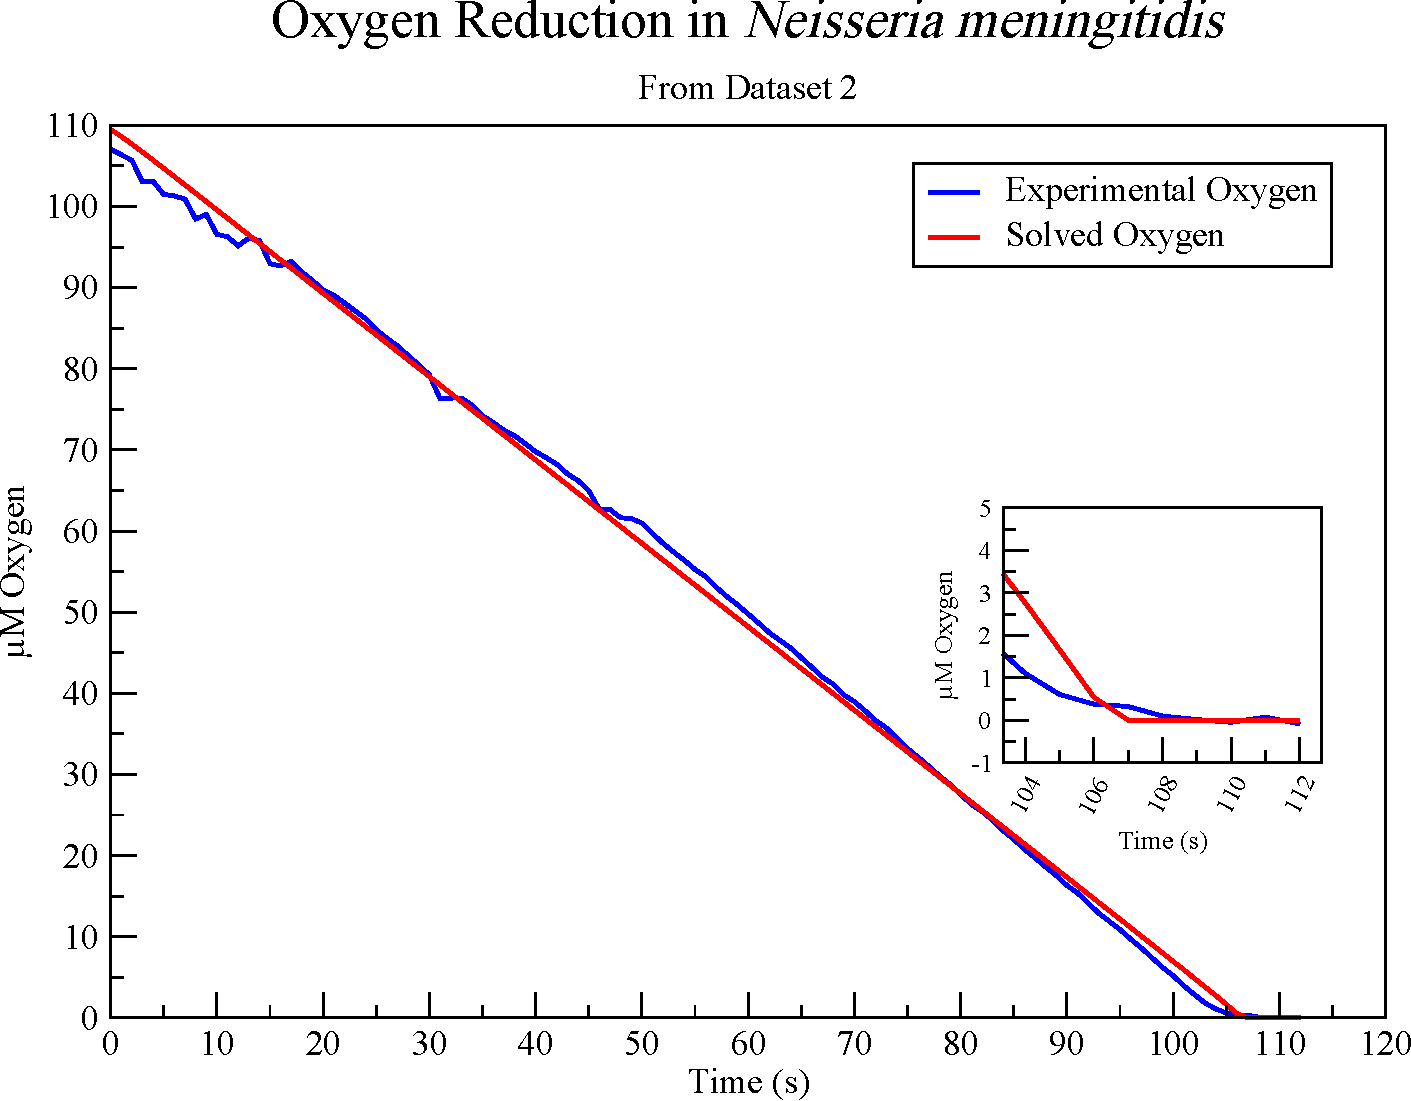
\includegraphics[width=14cm, trim=2cm 1cm 4cm 1cm]{./05-oxygenreduction/data/o2sim.pdf}
 % o2sim.eps: 0x0 pixel, 300dpi, 0.00x0.00 cm, bb=0 0 794 595
 \caption[{Oxygen Reduction in \textit{Neisseria meningitidis}.}]{{\bf Oxygen Reduction in \textit{Neisseria meningitidis}.} This dataset shows the simple linear reduction of Oxygen in aerobic conditions. The high affinity of $\mathrm{cbb}_3$ for oxygen is evidenced by very little non-linearity at low oxygen concentrations. The solved output is a representative result of the parameter estimation system.
 \label{fig:o2sim}}
\end{figure}

Initially the simulation results are not particularly good fits compared to the experimental data and as such have high ``fitness values''. As the parameter estimation progresses the ``fitness value'' reduces as the simulated result gets closer and closer to the experimental data. Quite often this does not take many iterations and a representative plot showing how the simulation's ``fitness value'' decreases is shown in Figure \ref{fig:oxy_fitness}. The initial period where the ``fitness value'' is high up until the point it settles at a lower value is classed as ``burn-in'' and is discarded when generating posterior distributions.

\begin{figure}[tbp]
 \centering
 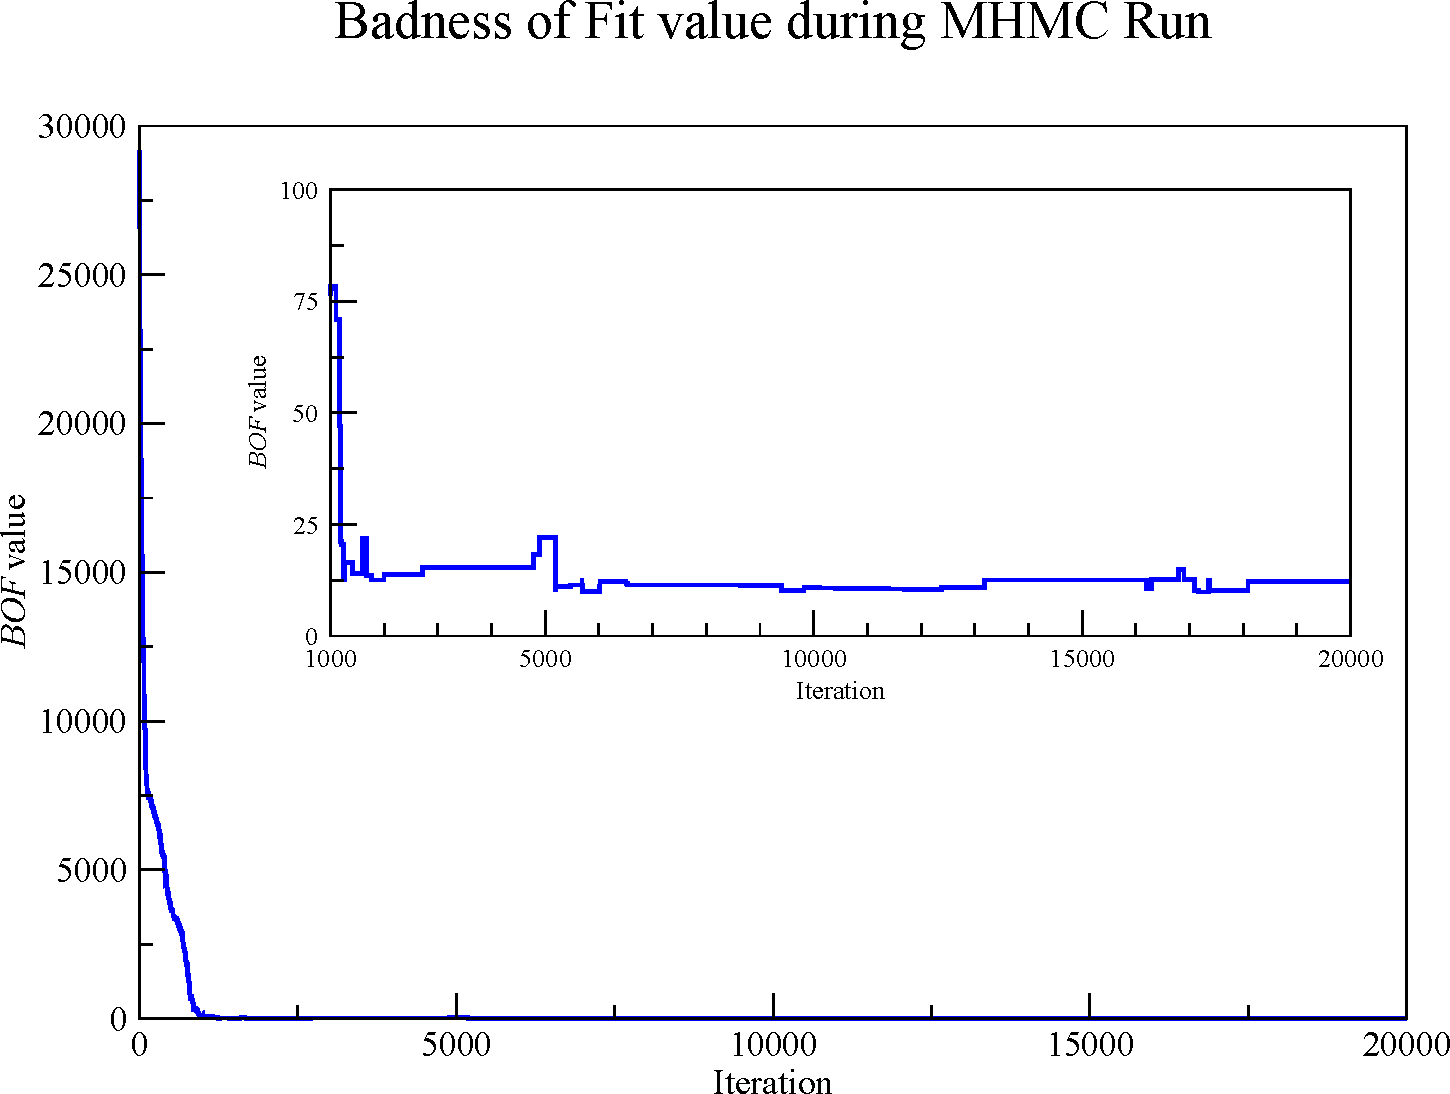
\includegraphics[width=14cm, trim=75px 50px 125px 25px]{./05-oxygenreduction/data/o2_fitness.pdf}
 % repeatable-oxygen-utilisation-in-mc58.png: 640x480 pixel, 72dpi, 22.58x16.93 cm, bb=0 0 640 480
 \caption[Simulation fitness value improves as parameter estimation progresses]{{\bf Simulation fitness value improves as parameter estimation progresses.} This is a representative figure constructed from a single run on one dataset. Initially the fitness value is high showing that the simulated result does not match the experimental dataset. As the parameter estimation algorithm progresses, the fitness value decreases as the simulated result approaches the experimental dataset. The inset shows a zoomed in view of the fitness value after the ``burn-in'' process has finished.
 \label{fig:oxy_fitness}}
\end{figure}

Each of the parameters that are to be estimated produces a trajectory of values for each run of the estimation algorithm. These trajectories are used to generate the posterior probability distributions required for Bayesian inference in subsequent steps. During the ``burn in'' period the parameter values can be observed to change rapidly from one iteration to the next as they approach their optimum values. Once the ``burn in'' has completed the values settle and produce largely flat trajectories with minor deviations around the optimum value. This settled region is used as the source for generating the posterior probability distributions. Figure \ref{fig:k3s} shows the the trajectories from each simulation run on a single dataset for the $k_3$ parameter. In this case the trajectory has been truncated to around 17000 iterations.

\begin{figure}[tbp]
 \centering
 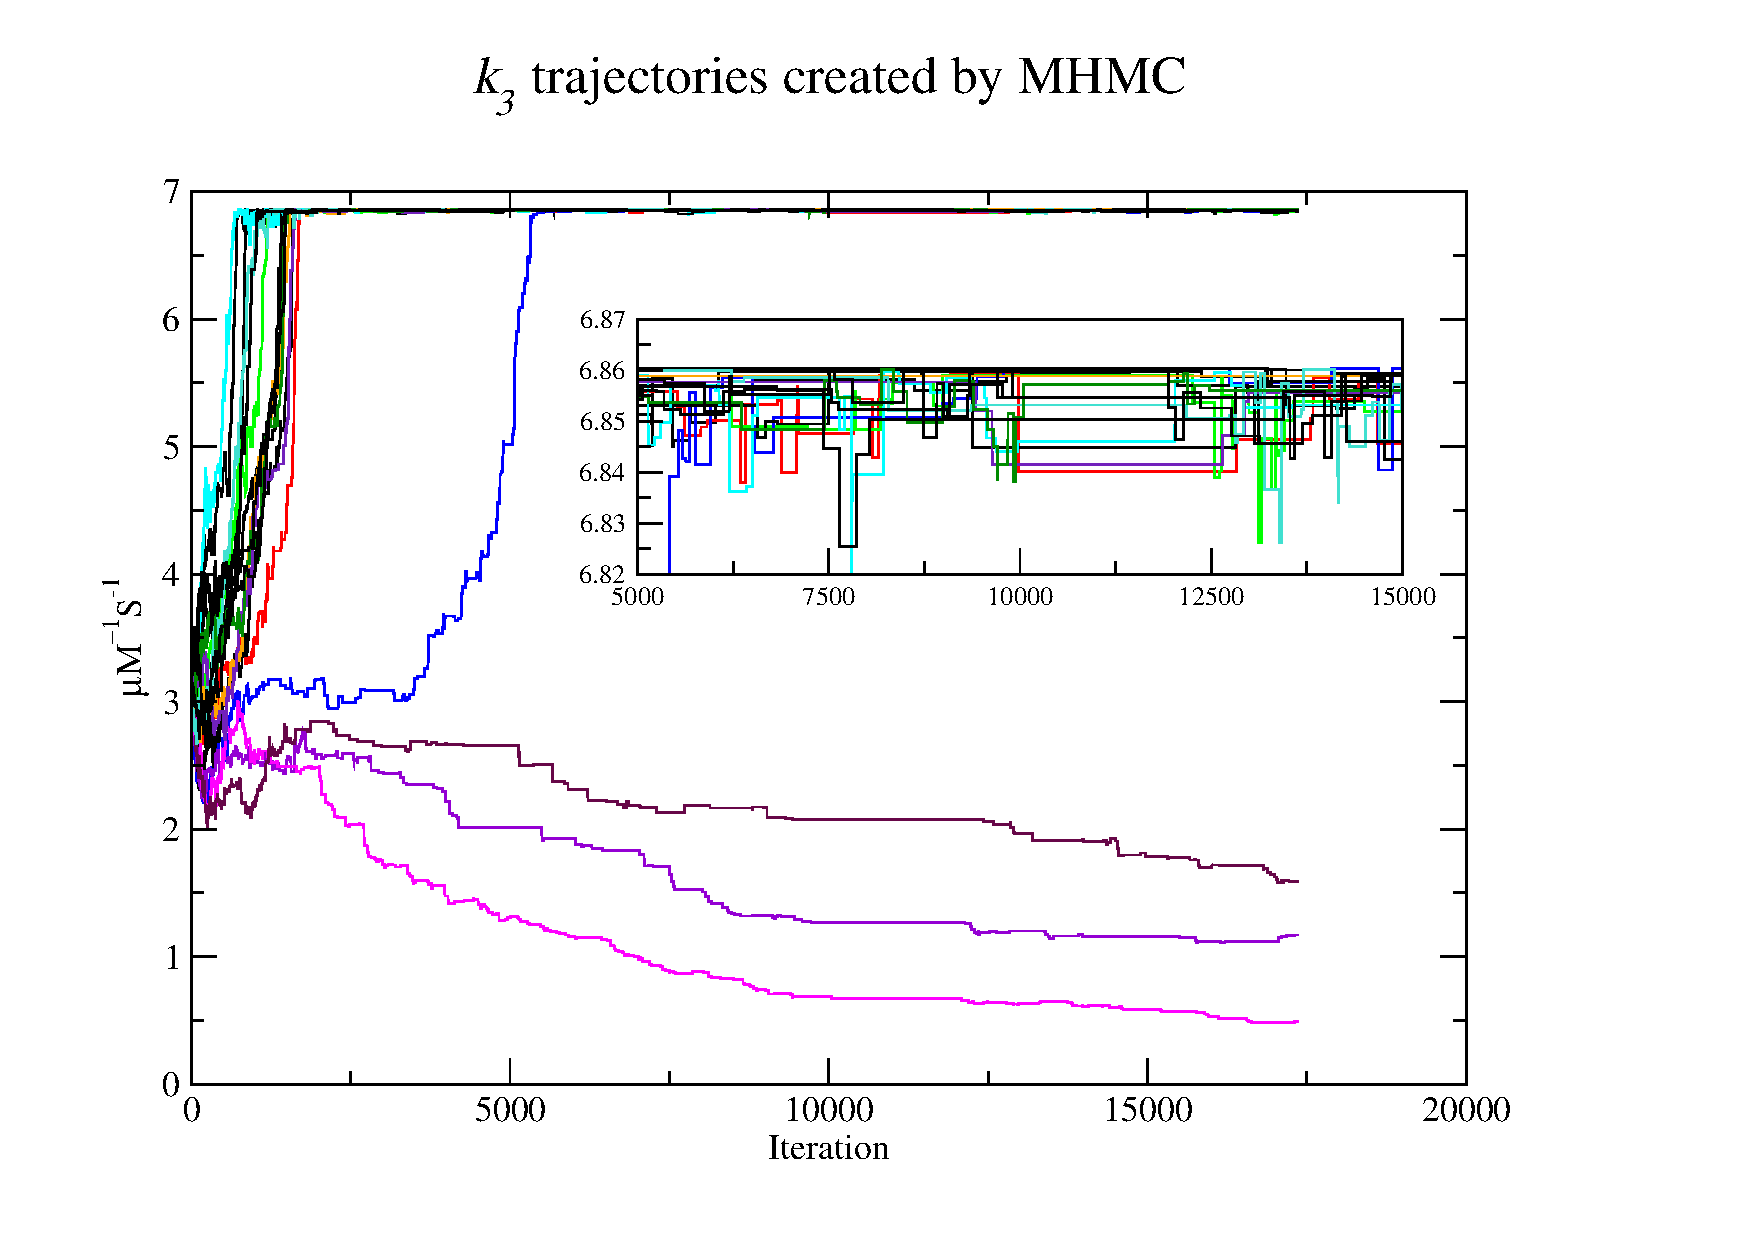
\includegraphics[width=14cm, trim=75px 50px 125px 25px]{./05-oxygenreduction/data/k3s.pdf}
 % repeatable-oxygen-utilisation-in-mc58.png: 640x480 pixel, 72dpi, 22.58x16.93 cm, bb=0 0 640 480
 \caption[Individual parameter trajectories for multiple runs on the same experimental dataset]{{\bf Individual parameter trajectories for multiple runs on the same experimental dataset.} This figure shows the trajectories for the same parameter, in this case $k_3$ - the rate of \cbbthree{} reduction, from 20 individual runs of parameter estimation upon the same input data. The inset shows a zoomed in view of the trajectories that hit high values after ``burn-in''.
 \label{fig:k3s}}
\end{figure}

Not all parameters in this stage of the model will produce trajectories like the one shown, as if there is a great deal of freedom as to what value a particular value can take without drastically increasing the ``fitness value'' it will be accepted by the parameter estimation algorithm. In this case the trajectories will not converge, and will ultimately produce a wide probability distribution. This is not necessarily indicative of a problem however, as this output still contains information that can be used in the next stage of parameter estimation with new datasets.

The trajectories above are processed to produce probability distributions given as histograms. The ``burn in'' is discarded and the settled data is then binned and counted. For the datasets used, the burn-in period differed and was filtered based on a pre-determined ``fitness value'' threshold. Datasets 1 \& 2 were had a threshold of $fv < 50.0$ and dataset 3 had a threshold of $fv < 90.0$. The reason for this difference is that dataset 3 never achieves a ``fitness value'' lower than about 80 due to noise in the experimental data. It is possible to assign these histogram probabilities as the posterior distributions and in turn use them directly as prior probability distributions for new datasets, however it was decided that given that the distribution around a particular value is likely to be normal, the histograms should be transformed into normal distribution probability density functions. This also has the advantage of allowing me to directly overlay the posterior probability distributions over the priors shown in Figure \ref{fig:oxypriors}.

The posterior probability distributions generated from the three experimental datasets, each started with 20 runs are shown in Figure \ref{fig:oxyposteriors}. In the case of parameters which represent concentrations, such as $X$ and $C$, the concentrations of cytochromes and \cbbthree{} respectively, the parameter distribution shown is the lower portion of the obtained distribution. As the initial oxygen reduction rates differed between these datasets (dataset 2 had a reduction rate about 5x higher than that of datasets 1 and 3) due to cell density differences (as reflected by experimental $OD_{600}$ measurements), the probability distributions were bimodal showing two distinct peaks one at roughly 5x the value of the other. Therefore the lower of the two peaks is shown, representing the oxygen reduction rate of datasets 1 and 3.

%FIXME -> bimodal probability distribution not shown
Additionally $k_1$, the rate of reduction of Oxygen by \cbbthree{} showed bimodality (not shown currently) \textit{and} a very broad range. The bimodal nature of this distribution was not matched in any of the other parameters. This parameter is the last rate in the ETC of oxygen reduction, so it is quite possible that the rate limiting steps are in the previous stages of the ETC and thus in the parameter estimation system $k_1$ essentially becomes ``free''.

Some of the posterior probability distributions appear to have expanded outside their prior bounds. I am fairly certain that this is not an error and that samples \textit{are} being taken from the prior distributions, but rather that the prior distributions were sufficiently incorrect that the penalty for selecting a parameter value from the prior distribution which is very unlikely is outweighed by the large decrease in ``fitness value'' that this affords.

\begin{figure}[tbp]
 \centering
 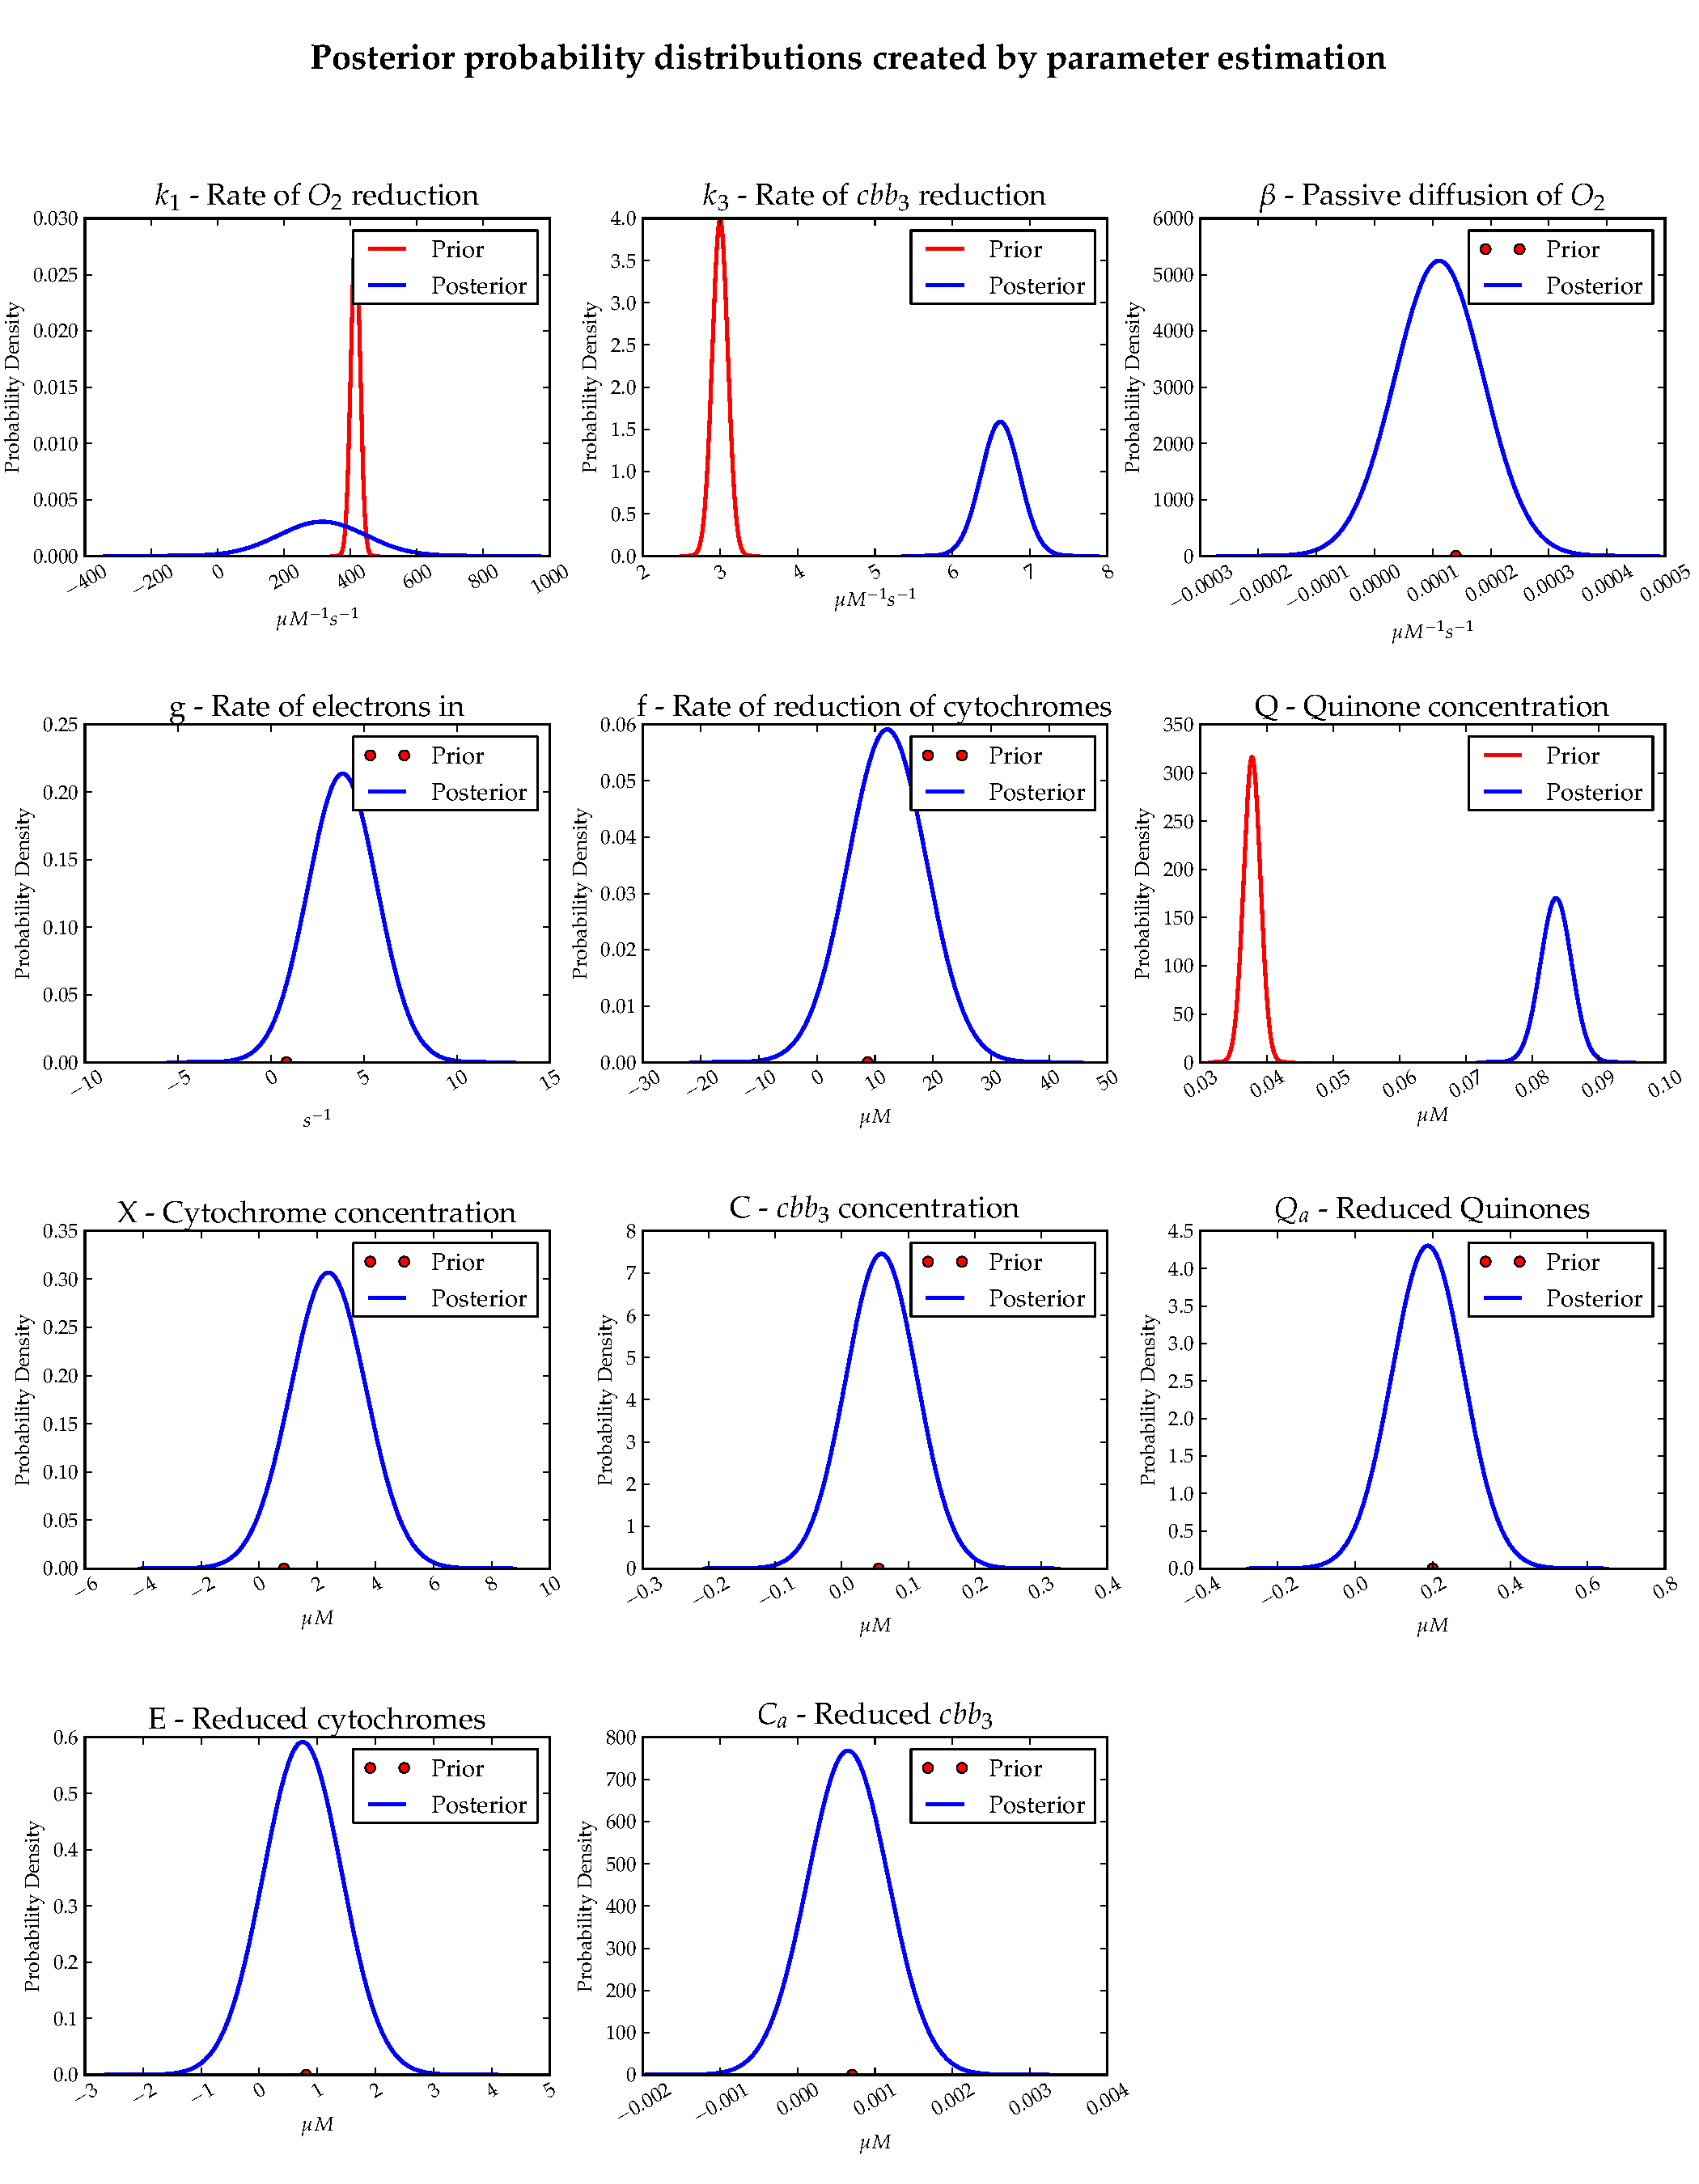
\includegraphics[width=15cm]{./05-oxygenreduction/data/posteriors.pdf}
 % posteriors.pdf: 1008x1008 pixel, 72dpi, 35.56x35.56 cm, bb=0 0 1008 1008
 \caption[Posterior probability distributions for oxygen reduction]{{\bf Posterior probability distributions for oxygen reduction}. These are the probability distributions generated by parameter estimation on 3 oxygen reduction datasets. These have been overlayed onto the prior probability distributions used by the parameter estimation algorithm, also shown in Figure \ref{fig:oxypriors}.
 \label{fig:oxyposteriors}}
\end{figure}

\subsubsection{Analysis of Convergence}
It is possible to calculate the degree of convergence of the parameters from the Monte Carlo trajectories using the R statistic introduced by \citet{Gelman1992}. This statistic produces in a single figure what could interpreted from the posterior probability distributions as it is essentially a measure of how close the trajectories have become towards the end of said trajectory. This statistic is calculated on the trajectories from multiple runs \textit{for each parameter individually}. The R statistic was calculated using the \textit{Bolstad2}\cite{Curran2011} library for R\cite{RDevelopmentCoreTeam2010}.

\subsubsection{Analysis of Correlation}
Given the large number of parameters, and the simple form of the experimental data it is quite likely that a number of the parameters will be correlated with one another. This effect should also be exacerbated at this stage due to the limited constraints (by virtue of wide prior probabilities) on the ranges of values that parameters can take. In order to investigate this I constructed a correlation matrix by calculating the Pearson's Product-Moment Correlation Coefficient for each of the parameters. This value provides the direction of correlation as indicated by the sign, and the degree of linearity as indicated by the magnitude. A positive correlation indicates that as the value of one parameter increases, the other increases also. A negative correlation indicates that as the value of one parameter increases, the other decreases.

The upper-triangle correlation matrix is shown in Figure \ref{tab:oxyregress} and was constructed by concatenating all the trajectories created by the parameter estimation system (discarding the burn-in) together and the Pearson's Product-Moment Correlation Coefficient calculated for each combination. The matrix is upper-triangle only as the lower triangle is a duplicate of the same data. The diagonal is shown in grey as it is not useful data since the correlation of X against X is always 1.

The correlation matrix shows that the majority of the parameters are not correlated with each other, giving very low $R^2$ values. A number of the parameters showed moderate correlation, which is to be expected. Parameters such as $k_1$ - the rate of reduction of oxygen - and $k_3$ - the rate of reduction of \cbbthree{} -  broadly speaking would increase as g - the rate of electrons in -  increased. This was expected as more electrons means higher observable rates are possible. Strong positive correlations exist between the concentrations of cytochromes (X), \cbbthree{}(C) and the rate of electrons in (g). This makes sense if the system wants to increase throughput of electrons but cannot do it by increasing the size of the quinone pool. Large numbers of electrons can be reduced by the cytochromes to eventually reduce oxygen.

Interestingly there were no negative correlations observed. This is somewhat odd as it might be expected that as the reduction rates of enzymes goes down, the concentration of the enzyme increases to maintain the same overall electron throughput. It appears however that the system is always trying to maximise oxygen throughput.

\begin{landscape}
\begin{table}[tbp]
\setlength{\tabcolsep}{5pt}
\renewcommand{\arraystretch}{1.5}
  \centering
  \begin{tabular}{|c|c|c|c|c|c|c|c|c|c|c|c|c|}
    \hline
    \cellcolor{dark-gray} & \cellcolor{dark-gray}$k_1$ & \cellcolor{dark-gray}$k_3$ & \cellcolor{dark-gray}$\beta$ & \cellcolor{dark-gray}g & \cellcolor{dark-gray}f & \cellcolor{dark-gray}Q & \cellcolor{dark-gray}X & \cellcolor{dark-gray}C & \cellcolor{dark-gray}$Q_a$ & \cellcolor{dark-gray}E & \cellcolor{dark-gray}$C_a$ \\
    \hline
    \cellcolor{dark-gray}$k_1$ & \cellcolor{light-gray}$1$ & $0.28599$ & $0.013212$ & \cellcolor{orange}$0.420123$ & $0.154821$ & $0.009968$ & \cellcolor{orange}$0.369637$ & \cellcolor{orange}$0.367247$ & $0.00344$ & $0.000229$ & $0.046062$ \\
    \hline
    \cellcolor{dark-gray}$k_3$ & \cellcolor{light-gray} & \cellcolor{light-gray}$1$ & $0.008486$ & \cellcolor{orange}$0.586606$ & \cellcolor{orange}$0.351956$ & $0.002927$ & \cellcolor{orange}$0.617929$ & \cellcolor{orange}$0.681098$ & $0.000559$ & $0.001062$ & $0.012978$ \\
    \hline
    \cellcolor{dark-gray}$\beta$ & \cellcolor{light-gray} & \cellcolor{light-gray} & \cellcolor{light-gray}$1$ & $0.009472$ & $0.07071$ & $6.58\times{}10^{-5}$ & $0.001034$ & $0.019449$ & $0.006711$ & $0.055052$ & $0.002166$ \\
    \hline
    \cellcolor{dark-gray}g & \cellcolor{light-gray} & \cellcolor{light-gray} & \cellcolor{light-gray} & \cellcolor{light-gray}$1$ & \cellcolor{orange}$0.426205$ & $0.008692$ & \cellcolor{green}$0.86507$ & \cellcolor{green}$0.811637$ & $0.009455$ & $0.003244$ & $0.076195$ \\
    \hline
    \cellcolor{dark-gray}f & \cellcolor{light-gray} & \cellcolor{light-gray} & \cellcolor{light-gray} & \cellcolor{light-gray} & \cellcolor{light-gray}$1$ & $0.00461$ & \cellcolor{orange}$0.329468$ & \cellcolor{orange}$0.432466$ & $0.106478$ & $0.012951$ & $0.001404$ \\
    \hline
    \cellcolor{dark-gray}Q & \cellcolor{light-gray} & \cellcolor{light-gray} & \cellcolor{light-gray} & \cellcolor{light-gray} & \cellcolor{light-gray} & \cellcolor{light-gray}$1$ & $0.008756$ & $0.006046$ & $0.00024$ & $7.86\times{}10^{-6}$ & $0.003555$ \\
    \hline
    \cellcolor{dark-gray}X & \cellcolor{light-gray} & \cellcolor{light-gray} & \cellcolor{light-gray} & \cellcolor{light-gray} & \cellcolor{light-gray} & \cellcolor{light-gray} & \cellcolor{light-gray}$1$ & \cellcolor{green}$0.803124$ & $1.47\times{}10^{-5}$ & $3.43\times{}10^{-5}$ & $0.064213$ \\
    \hline
    \cellcolor{dark-gray}C & \cellcolor{light-gray} & \cellcolor{light-gray} & \cellcolor{light-gray} & \cellcolor{light-gray} & \cellcolor{light-gray} & \cellcolor{light-gray} & \cellcolor{light-gray} & \cellcolor{light-gray}$1$ & $0.018731$ & $7.27\times{}10^{-5}$ & $0.046421$ \\
    \hline
    \cellcolor{dark-gray}$Q_a$ & \cellcolor{light-gray} & \cellcolor{light-gray} & \cellcolor{light-gray} & \cellcolor{light-gray} & \cellcolor{light-gray} & \cellcolor{light-gray} & \cellcolor{light-gray} & \cellcolor{light-gray} & \cellcolor{light-gray}$1$ & $0.108255$ & $0.00897$ \\
    \hline
    \cellcolor{dark-gray}E & \cellcolor{light-gray} & \cellcolor{light-gray} & \cellcolor{light-gray} & \cellcolor{light-gray} & \cellcolor{light-gray} & \cellcolor{light-gray} & \cellcolor{light-gray} & \cellcolor{light-gray} & \cellcolor{light-gray} & \cellcolor{light-gray}$1$ & $0.003167$ \\
    \hline
    \cellcolor{dark-gray}$C_a$ & \cellcolor{light-gray} & \cellcolor{light-gray} & \cellcolor{light-gray} & \cellcolor{light-gray} & \cellcolor{light-gray} & \cellcolor{light-gray} & \cellcolor{light-gray} & \cellcolor{light-gray} & \cellcolor{light-gray} & \cellcolor{light-gray} & \cellcolor{light-gray}$1$ \\
    \hline
  \end{tabular}
  \caption[Regression Analysis of Oxygen Reduction Parameters]{{\bf Regression Analysis of Oxygen Reduction Parameters.} This table shows the $R^2$ values from linear regression analysis on the combined parameter trajectories for Oxygen reduction. Parameters with high correlation have been coloured green ($R^2>0.8$) and those with moderation correlation have been coloured orange ($0.8>R^2>0.3$).
  \label{tab:oxyregress}}
\end{table}
\end{landscape}

\setlength{\tabcolsep}{6pt}

\subsection{Rate of oxygen diffusion}
During the course of this experimental stage I noticed that on occasions where the respiring cultures died, either through being left in essentially anaerobic conditions for too long, or intentionally killed with Chloramphenicol, the oxygen levels in the culture media would begin to rise slowly. This did not occur in every case, and after some further experimentation I concluded that it probably occurs when an air bubble gets trapped underneath the lid of the oxygen electrode chamber. The average rates of oxygen diffusion were very small, and on the experimental time-scales are probably negligible, but I thought it necessary to include in the model for completeness.

The equation used to fit raw data for oxygen diffusion is a 3 parameter exponential:
\begin{equation*}
f(x) = c - ae^{-bx} 
\end{equation*}
In the differential equation this collapses to two parameters, the oxygen saturation level, and the rate of oxygen recovery thus:
\begin{equation*}
\dfrac{d[O_2]}{dt} = \beta(1-O_2/K_O)
\end{equation*}
Integrating and separating this equation gives:
\begin{equation*}
\begin{gathered}
-\beta\dfrac{t}{K_O} + C = ln([O_2]-K_O)\\
\Rightarrow [O_2]-K_O = Ae^{\left(-\beta\dfrac{t}{K_O}\right)}\\
\Rightarrow [O_2] = K_O + Ae^{\left(-\beta\dfrac{t}{K_O}\right)}
\end{gathered}
\end{equation*}

\subsection{Discussion}
The experimental dataset shows that oxygen reduction in \textit{Neisseria meningitidis} is a simple linear system with the reductase having a high affinity for oxygen demonstrated by the almost complete lack of non-linearity as oxygen concentration approaches zero. This apparent simple linearity could be modelled with a high degree of accuracy with just 2 parameters in a simple $y=-mx+c$ system. However this does mean that the posterior distributions generated are very wide and therefore allows much greater freedom for the next dataset to explore the parameter space.

Given the knowledge of the underlying transport chain and the affinity of \cbbthree{} for oxygen, I expected a linear reduction of oxygen with high affinity over nearly two orders of magnitude. It is however remarkable that I can model this behaviour with so few components in the model, as it requires significant changes in the reduction state of the enzymes to achieve this.